\mysubsection{Calendrier du projet}

Afin d’analyser et gérer le progrès de l’équipe et l'exécution des différentes tâches, on a fait l’estimation de la durée d’exécution des activités nécessaires pour la conclusion du projet. La table \ref{fig:cronograma1} décrit le calendrier de réalisation du projet.

\begin{figure}[H]
	\begin{center}	
		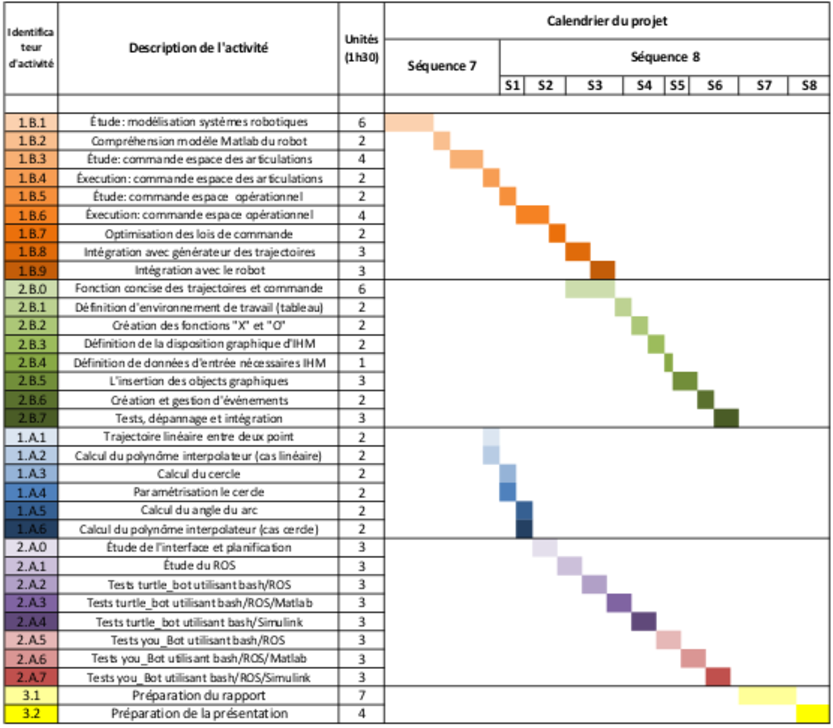
\includegraphics[width=\textwidth]{./Cronograma1}
		\caption{Calendrier de réalisation du projet.}
		\label{fig:cronograma1}
	\end{center}
\end{figure}

Les unités de temps sont considérés en créneaux, où chaque créneau correspond à une durée de 1h30. Pour les jours dans lesquels seulement la moitié de l’équipe est présente dans le laboratoire, on a considéré la moitié du temps de chaque créneaux. 
On 54 créneaux au total pour la conclusion du projet.
